% M. S. Tsoeu (2011), University of Cape Town <mohohlo.tsoeu@uct.ac.za>

% This is a project report templace document created for EEE4022FS students at the University of Cape Town.
%
% This file should be is processed with ``pdflatex`` and might need a few modifications if a different processor is chosen.


\documentclass[a4paper,12pt]{report}

%Include packages you need to use here

\usepackage[top = 1in, bottom = 1in, left = 1in, right = 1in]{geometry}
\usepackage{graphicx}
\usepackage{fancyhdr}
\usepackage{amsmath, amsthm, amssymb}
\usepackage{lastpage}
\usepackage{subfigure}
\usepackage{lscape}
\usepackage{hyphenat}
\usepackage{setspace}
\usepackage{hyperref}
\newcommand{\algorithmautorefname}{Algorithm} % give hyperref or \autoref a name for algorithms
\usepackage{gensymb} % for \degree
\usepackage{algorithm} % for algorithm float
\usepackage{algpseudocode} % for pseudocode
\renewcommand{\algorithmiccomment}[1]{\hfill // #1} % make comments //
% \newcommand{\LineComment}[1]{\Statex \hspace*{\algorithmicindent}\hspace{1em} // #1} % add comments on its own line
% \newcommand{\LineComment}[2][1]{\State\hspace{#1\algorithmicindent}#2}
\newcommand{\LineComment}[2][0]{\Statex \hspace*{\algorithmicindent}\hspace{#1em} // #2} % add comments on its own line
\DeclareMathOperator{\sgn}{sgn} % sign function

% Include page formatting here. 
\parskip = 6mm
\parindent = 0mm
\renewcommand{\headrulewidth}{0pt}
\rhead[]{\thesection}
\lhead[\thechapter]{}

% Reduce space below Chapter and Section headings
\usepackage{titlesec}
\titlespacing*{\chapter}{0pt}{0ex}{0ex} % Chapters
\titlespacing*{\section}{0pt}{0ex}{0ex} % Sections

\begin{document}
 
% This section formats the title page of the Report.
\thispagestyle{empty}
{\Huge \begin{center}
% Modify the line below to insert your title.
Insert your title here
\hrule 
% Modify the line below to insert your subtitle.
{\Large Insert a subtitle here (if applicable)}
\end{center}}

\vskip 5mm
\begin{center}
\- \- \- \- \- \- \- \- \- \-
\includegraphics[scale = 0.3]{graphics/uctLogo.png}
\end{center}

\vskip 5mm
\begin{center}
Presented by:\\
Mohohlo Samuel T\v soeu		% Insert your name here
\end{center}

\vskip 10mm
\begin{center}
Prepared for:\\
M. S. T\v soeu\\ 		% Insert your supervisor's name here.
Dept. of Electrical and Electronics Engineering\\University of Cape Town
\end{center}


\vskip 10mm
\begin{center}
Submitted to the Department of Electrical Engineering at the University of Cape Town in partial
fulfilment of the academic requirements for a Bachelor of Science degree in ***INSERT DEGREE
NAME HERE (Electrical Engineering; Mechatronics or Electrical and Computer Engineering)

\end{center}


\vskip 5mm
\begin{center}{\bf \today}
\end{center}


\newpage
\thispagestyle{empty}
\mbox{}

\onehalfspacing
\nohyphens{
\thispagestyle{empty}
\vskip 40mm

\newpage
% Please leave the declaration as it is (Standard UCT declaration).
{\Large Declaration}\\
\hrule

\vskip 10mm
\begin{enumerate}
\item I know that plagiarism is wrong. Plagiarism is to use another's work and pretend that it is one's own.
\item I have used the \underline{IEEE} convention for citation and referencing. Each contribution to, and quotation in, this report from the work(s) of other people has been attributed, and has been cited and
referenced. Any section taken from an internet source has been referenced to that source.
\item This report is my own work, and is in my own words (except where I have attributed it to others).
\item \textbf{I have not paid a third party to complete my work on my behalf. My use of artificial intelligence software has been limit to \underline{[see \autoref{app:AI_usage}]} (specify precisely how you used AI to assist with this assignment).}
\item I have not allowed and will not allow anyone to copy my work with the intention of passing it off as his or her own work.
\item I acknowledge that copying someone else's assignment or essay, or part of it, is wrong, and declare that this is my own work.
\end{enumerate}
\vskip 10mm
Signature:\ldots\ldots\ldots\ldots\ldots\ldots\ldots\ldots\ldots 
\\ N. Vorsatz 		% Change this line to your name.
\vskip10mm
Date:\ldots\ldots\ldots\ldots\ldots\ldots\ldots\ldots\ldots\ldots
\vskip10mm
Word count: 8418\\
(excl. headings, tables, figures, equations and footers)

\newpage
\thispagestyle{empty}
{\Large Terms of Reference}\\
\hrule

The terms of reference page is an agreement between yourself and your supervisor outlining what is expected of you in your final year project. Please make sure that this is discussed and written at the beginning of your thesis project. 

\fancyfoot[C]{\thepage}
\pagestyle{plain}
\newpage
\pagenumbering{roman}
{\Large Acknowledgments}\\
\hrule
% Make relevant acknowledgements to people who have helped you complete or conduct this work, including sponsors or research funders.
I send my thanks to my supervisor, A/Prof Ramotsoela, for keeping me ontrack with completing this project's goals, as opposed to drifting off on a tangent.

I send my thanks to Shaun Beautement for bringing to my attention the Hairy Ball Theorem, and its implications on a static kinematic mapping.

I send my thanks to Lusango Mbongo for developing the initial designs of the 3D printed mount, which holds the Braccio and attached modules.

I send my thanks to an anonymous person for recommending that I look into virtual private networks.

Lastly, I send my thanks to my friends and family, who all indirectly supported this project.

Oh yes- let's not forget Budget Rolls, for being my primary source of nourishment during long days on upper campus. I recommend trying their \textit{chicken tikka avo sandwiches} if given the chance. (I'm not sponsored by them, and don't take on any liability in giving this recommendation.)

\newpage
{\Large Abstract}\\
\hrule

% Place your abstract here.
% \begin{itemize}
% \item Open the {\bf Project Report Template.tex} file and carefully follow the comments (starting with \%).
% \item Process the file with {\bf pdflatex}, using other processors may need you to change some features such as graphics types.
% \item Note the files included in the  {\bf Project Report Template.tex} (with the .tex extension excluded). You can open these files separately and modify their contents 
% or create new ones.
% \item Contact the latex namual for more features in your document such as equations, subfigures, footnotes, subscripts \& superscripts, special characters etc.
% \item I recommend using the {\bf kile} latex IDE, as it is simple to use.
% \end{itemize}

Teleoperation systems are used to allow humans to control robotic systems over large distances. An ideal user experience involves non-intrusive sensing and intuitive spatial mapping. Few implementations of teleoperation discuss the effects of applying cybersecurity principles to the resource constrained hardware inherent to some robotic systems. This report discusses the implementation of an intuitive and non-invasive teleoperation system, using computer vision, while keeping network security and constraints in consideration. The system uses a pre-trained computer vision pipeline, along with an inverse kinematics algorithm to determine the actuation values for a Tinkerkit Braccio. Packets sent from the operator-side to the Braccio-side are managed by the DTLS protocol, using pre-shared keys. Due to monocular depth ambiguity, the motion of the Braccio was constrained to 2 dimensions. Through experiments, it was found that the smoothing algorithm used to reduce aggressive movements contributed most ($88.3\%$) to the system's total latency. The latency due to encryption and decryption were otherwise insignificant, and this is more apparent over slower networks, such as due to large geographical separation. The implementation code, report source code, raw data and videos can all be found on the project's \href{https://github.com/Neo-Vorsatz-UCT/eee4022s}{GitHub}.


\newpage
\tableofcontents

%\newpage
%\listoffigures

%\newpage
%\listoftables

% Page formatting, to place section titles as headers of odd pages and Chapter titles as headers of even pages.
\newpage
\fancyhead[RE,LO]{}
\fancyhead[LE]{\leftmark}
\fancyhead[RO]{\rightmark}
\pagestyle{fancy}

\pagenumbering{arabic}

% THe files included below are .tex files containing the respective chapters these are already created in this package and you can add to or modify them.
\chapter{Introduction}

\section{Background to the project}
% A very brief background to your area of research. Start off with a general introduction to the area and
% then narrow it down to your focus area. Used to set the scene \cite{smt2011}.
Teleoperation is the control of systems (often robotic) over large distance. This is done because it's often useful to have a human in the loop as opposed to fully automated systems. Teleoperation poses many modern challenges, such as keeping the network secure and responsive on resource constrained hardware. Non intrusive and intuitive methods of reading user input, such as computer vision, are also preferred because they introduce less fatigue and strain on the operator.

\section{Objectives of this project}
% \subsection{Problems to be investigated}
% Description of the main questions to be investigated in this study.
This project aims to develop a teleoperation system using the Tinkerkit Braccio for Arduino and an ESP32, by implementing non-intrusive computer vision to read user input, and keeping the network security in mind.

% \subsection{Purpose of the project}
% Give the significance of investigating these problems. It must be obvious why you are doing this study
% and why it is relevant.
This is done to demonstrate and investigate the use of computer vision and intuitive control schemes in teleoperation systems. This project also discusses the overall cybersecurity of this system, and investigates the effects of implementing cybersecurity principles on the network's performance, given resource constrained hardware.

\section{Scope and Limitations}
% Scope indicates to the reader what has and has not been included in the study. Limitations tell the
% reader what factors influenced the study such as sample size, time etc. It is not a section for excuses as
% to why your project may or may not have worked.
This project assumes an ideal operator environment, where the robustness of the computer vision is not a concern.\\
This project does not implement a feedback system for the operator, and hence assumes the operator already has some way to see the slave's and its environment.\\
This project also focuses on the implementation of cybersecurity for the internet traffic, as other security such as for the hardware or encryption keys would not significantly affect the performance of the teleoperation.\\
This project does not investigate the overall accuracy of the teleoperation.

\newpage
\section{Plan of development}
% Here you tell the reader how your report has been organised and what is included in each
% chapter.

% {\bf I recommend that you write this section last. You can then tailor it to your report.}
In \autoref{ch:lit}, is a review of similar projects and studies, and the technologies surrounding the subsystems for this project.

From \autoref{ch:comp_vis} to \autoref{ch:act} are the explanations of the design and implementation of each of this project's subsystems:
\begin{itemize}[nosep]
    \item \autoref{ch:comp_vis} is dedicated to the computer vision subsystem, explaining how user input is taken and interpreted.
    \item \autoref{ch:ik} goes through the implementation of the inverse kinematics subsystems, which maps the desired end-effector target to a set of actuation/control values for the Braccio.
    \item \autoref{ch:net} discusses some risks the network faces, and how those risks were mitigated in the networking system.
    \item \autoref{ch:act} explains how the Braccio was actuated to achieve the desired end-effector target.
\end{itemize}

The results are shown and discussed in \autoref{ch:re} and \autoref{ch:dis}. The outputs of this project are summarised in \autoref{ch:conc}, and recommendations for future work are made in \autoref{ch:rec}.

\vspace{2em}
\hrule

\chapter{Literature Review}

% Once upon a time engineers and researchers believed... In this area of research, they used the following methods... \cite{jct2010}

% Write this section first as it will take you the longest. I suggest you start writing this as soon as you
% have done your initial research at the beginning of your project. You can then return to it once you
% have completed your work to edit and adjust it.

% A literature review forms the theoretical basis of your project. You need to read a large number of
% journal papers, sections in books, technical reports etc. relevant to your work at the start of project.
% This will give you a good idea of the field of research.

% When writing your review start of with the general concepts and move to the more specific aspects
% explaining the necessary theory as you go. This section is NOT a copy and paste from others work or a
% rewrite-but-change-one-word section. I suggest you read all your material, and then put it down and
% write this section, referring back to the work only when you need to check something.

% See your PCS textbook for more details on how to write a literature review.

% If you include a figure or a table in your text please see the example in Fig. \ref{fig:model} as to how to caption it.
% Please make sure that all text in your figures is readable and that you reference your figures if they are
% from another source.

% \begin{figure}[ht]
% \centering
% 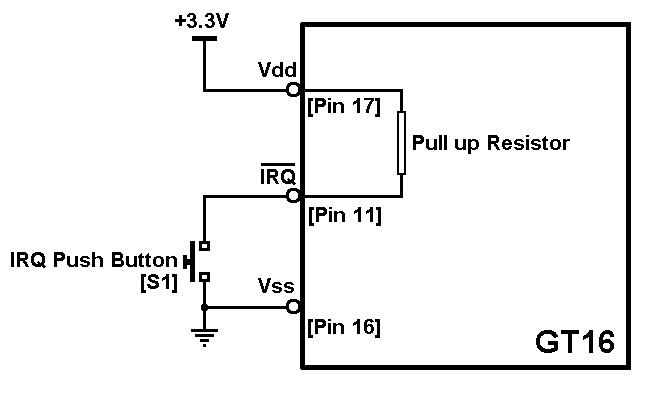
\includegraphics[width=0.7\textwidth]{graphics/model.png}
% \caption{A block diagram illustrating the connections to the IRQ pin on the MCS08GT16A microcontroller (Please
% note that your headings should be short descriptions of what is in the diagram not simply the figure title)}
% \label{fig:model}
% \end{figure}

\section{Tinkerkit Braccio arm for Arduno}
The Braccio arm has been used in similar projects to demonstrate teleoperation via intuitive control (natural human motions). An example uses an armband to measure the muscle contractions of a human arm \cite{bib:braccio_armband_demo}.

The Braccio arm has also been used in other projects. For a feeding-assistant, the engineers used Denavit-Hartenberg parameters and forward-kinematics to determine the position of the end-effector \cite{bib:braccio_feeding_assistant}. The Denavit-Hartenberg parameters used in the study are shown in \autoref{tab:lit_dh_parameters}.

\begin{table}[h!]
\centering
\caption{Denavit-Hartenberg parameters for Braccio arm}
\label{tab:lit_dh_parameters}
\begin{tabular}{|c|c|c|c|c|}
    \hline
    \textbf{i} & \textbf{$\alpha_{i-1}$ (degrees)} & \textbf{$r_{i-1}$ (inches)} & \textbf{$d_{i}$ (inches)} & $\theta_{i}$ (degrees) \\
    \hline \hline
    1 & 0 & 0 & 0 & $\theta_1$ \\
    \hline
    2 & 90 & 0 & 0 & $\theta_2$ \\
    \hline
    3 & 0 & 5 & 0 & $\theta_3$ \\
    \hline
    4 & 0 & 5 & 0 & $\theta_4$ \\
    \hline
    5 & 0 & 12 & 0 & $\theta_5$ \\
    \hline
\end{tabular}
\end{table}

There was a project involving the use of computer vision to control the Braccio arm \cite{bib:braccio_hand_gestures}. In this project, a camera connected to a Raspberry Pi would detect hand gestures (number of fingers being held up) from the user, and translate these into commands for the Braccio arm.

\section{Teleoperation}
Teleoperation has generally been in three categories \cite{bib:teleoperation_continuous_space}:
\begin{itemize}
    \item Joint mapping: Each joint of the slave device is mapped to a joint of the master device. This is only applicable if the kinematics are similar, which is not the case for a human arm and the Braccio arm.
    \item End-effector mapping: The end-effector of the slave device is mapped to the end-effector of the master, and the intermediate joints are determined with forward and inverse kinematics.
    \item Pose mapping: The general intention of the master device is mapped to the slave device.
\end{itemize}
The paper found that pose mapping, using a linear transformation in an intermediate space, was not only simpler to implement, but also more intuitive to use. The measure of "intuitiveness" comes from how quickly a novice was able to complete a task.

\section{Computer Vision}

The works of Moeslund and Granum \cite{bib:computer_vision_overview} summarises the advancements of computer vision in human tracking, from 1980 up till halfway through year 2000. The paper classifies human tracking into three applications; surveillance, control and analysis. From the descriptions given, control is what's relevant to this project.

The paper lists some common assumptions made in the context of computer vision. Computer vision isn't the focus of this project, so as many assumptions as applicable will be made, namely:
\begin{itemize}
    \item The subject (human arm) remains inside the workspace
    \item No camera motion
    \item Only one person in the workspace at the time
    \item No occlusion
    \item The motion pattern of the subject is known
    \item Minimal changes to lighting
    \item Static/uniform background
    \item Known camera parameters
\end{itemize}
That being the case, robustness of a tracking algorithm is not as much of a priority, compared to accuracy and speed.

The paper also discusses different ways of modelling the hand, from different abstraction methods. The stick-figure model, with joint-abstraction stands out, because it can most easily be translated into a corresponding pose for the Braccio arm.

% \chapter{Methodology}

% This is what I did to test and confirm my hypothesis.


% You may want to split this chapter into sub chapters depending on your design. I suggest you change
% the title to something more specific to your project.

% This is where you describe your design process in detail, from component/device selection to actual
% design implementation, to how you tested your system. Remember detail is important in technical
% writing. Do not just write I used a computer give the computer specifications or the oscilloscopes part
% number. Describe the system in enough detail so that someone else can replicate your design as well
% as your testing methodology.

% If you use or design code for your system, represent it as flow diagrams in text.

% \textbf{IMPORTANT:} Include a motivation for your selection of an appropriate technique, or engineering or IT tool to solve your project problem. Discuss any limitations if appropriate.
\chapter{Design}

\section{Kinematic Mapping}

\begin{algorithm}
\caption{Forward Reaching Algorithm}\label{alg:backward_reaching}
\begin{algorithmic}[1]
    \Require A sorted array $A$ of size $n$, and a target value $T$
    \Ensure The index of $T$ in $A$, or $-1$ if not found
    
    \Function{ForwardReaching}{$J$}
    \State $C\gets J.child$
        \If {$C$ is a hinge}
            \State $\vec{d}\gets C.\vec{pos}-J.\vec{pos}$
            \LineComment[1]{Project $\vec{d}$ onto the plane perpendicular to $C.\vec{axis}_{aux}$}
            \State $\vec{l}\gets\vec{d}-(\vec{d}\cdot C.\vec{axis}_{aux})C.\vec{axis}_{aux}$
            \State $mag\_l \gets |\vec{l}|$
            \LineComment[1]{Update joint orientation}
            \If {$mab\_l=0$}
                \State $J.\vec{axis}_{link}\gets C.\vec{axis}_{link}$
            \Else
                \State $J.\vec{axis}_{link}\gets\vec{l}/|\vec{l}|$
            \EndIf
            \State $J.\vec{axis}_{aux}\gets C.\vec{axis}_{aux}$
            \LineComment[1]{Check joint limits}
            \State $dir\gets\sgn((J.\vec{axis}_{link}\times C.\vec{axis}_{link})\cdot J.\vec{axis}_{aux})$
            \State $C.value\gets\cos^{-1}(J.\vec{axis}_{link}\cdot C.\vec{axis}_{link})dir$
            \If {$C$ is limited}
                \If {$C.value>C.high$}
                    \State $C.value\gets C.high$
                    \State $J.\vec{axis}_{link}\gets C.\vec{axis}_{link}\cos(C.value)$
                    \State $J.\vec{axis}_{link}\gets J.\vec{axis}_{link}+(C.\vec{axis}_{link}\times C.\vec{axis}_{aux})\sin(C.value)$
                \ElsIf {$C.value<C.low$}
                    \State $C.value\gets C.low$
                    \State $J.\vec{axis}_{link}\gets C.\vec{axis}_{link}\cos(C.value)$
                    \State $J.\vec{axis}_{link}\gets J.\vec{axis}_{link}+(C.\vec{axis}_{link}\times C.\vec{axis}_{aux})\sin(C.value)$
                \EndIf
            \Else
                \LineComment[1]{Argument angle}
                \State $C.value\gets\mod(C.value,360\degree)$
                \If {$C.value>180\degree$}
                    \State $C.value\gets C.value-360\degree$
                \EndIf
            \EndIf
            \LineComment[1]{Update joint position}
            \State $J.\vec{pos}\gets C.\vec{pos}-J.\vec{axis}_{link}J.len_{link}$
            \Statex

        \ElsIf {$C$ is a pivot}
            \State $J.\vec{axis}_{link}\gets C.\vec{axis}_{link}$
            \State $J.\vec{pos}\gets C.\vec{pos}-J.\vec{axis}_{link}J.len_{link}$
            \Statex

        \ElsIf {$C$ is prismatic}
            \State $J.\vec{axis}_{link}\gets C.\vec{axis}_{link}$
            \State $\vec{d}\gets C.\vec{pos}-J.\vec{pos}$
            \State $C.value\gets\vec{d}\cdot J.\vec{axis}_{link}$
            \LineComment[1]{Check joint limits}
            \If {$C$ is limited}
                \If {$C.value>C.high$}
                    \State $C.value\gets C.high$
                \ElsIf {$C.value<C.low$}
                    \State $C.value\gets C.low$
                \EndIf
            \EndIf
            \State $J.\vec{pos}\gets C.\vec{pos}-J.\vec{axis}_{link}C.value$
        \EndIf
        

    \EndFunction
\end{algorithmic}
\end{algorithm}

\chapter{Results}\label{ch:re}
% These are the results I found from my investigation.

% Present your results in a suitable format using tables and graphs where necessary. Remember to refer
% to them in text and caption them properly.


% \section{Simulation Results}


% \section{Experimental Results}

All raw data can be found on \href{https://github.com/Neo-Vorsatz-UCT/eee4022s/blob/main/data/}{GitHub}.

\section{Latency}
The latency of the system due to each stage of the pipeline is shown in \autoref{fig_re:latency_boxplot} as a box and whisker plot. The mean and standard deviation of these latencies, as well as the total are shown in \autoref{tab_re:latency_table}.\\
The step response of the Braccio, approximated to 10\degree\space steps is shown in \autoref{fig_re:braccio_step}, along with a spline fit using $\lambda=2$ to help visualise the step.

\begin{figure}[h!]
    \centering
    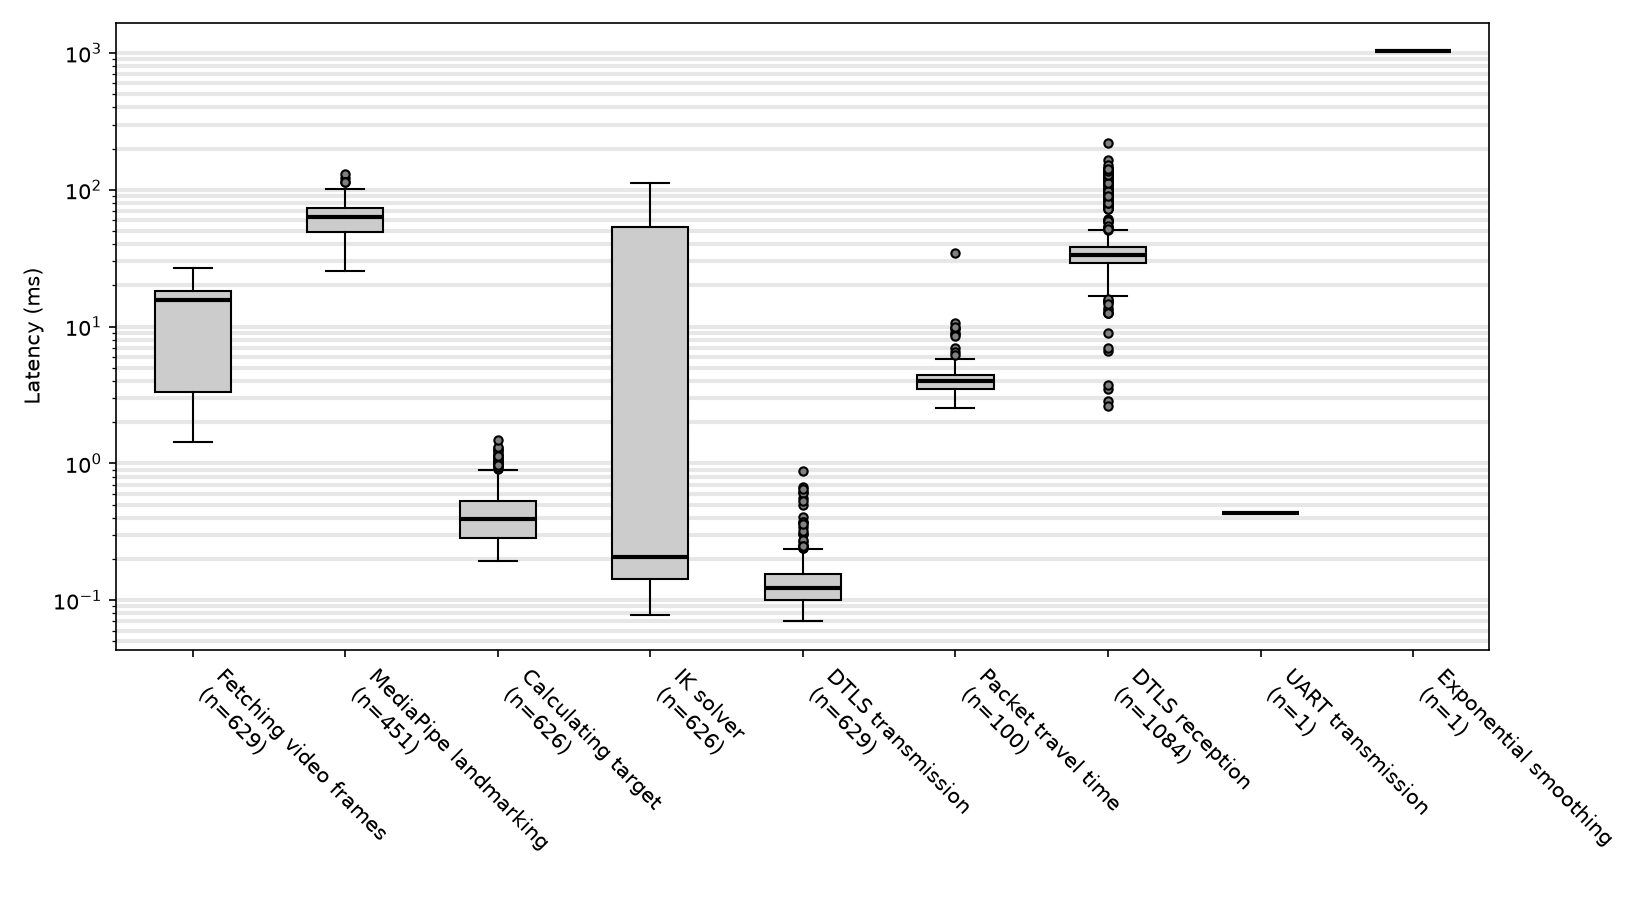
\includegraphics[width=1\textwidth]{graphics/results/latency_boxplot.png}
    \caption{Box and Whisker plot of latency contributed by each stage}
    \label{fig_re:latency_boxplot}
\end{figure}

\newpage
\begin{table}[h!]
\centering
\caption{Table of latency contributed by each stage}
\label{tab_re:latency_table}
\small{
\begin{tabular}{|l|c|c|c|c|}
    \hline
    \textbf{Stage} & \textbf{Mean (ms)} & \textbf{Standard Dev. (ms)} & \textbf{Number of Samples} & \textbf{Percentage of Total} \\
    \hline \hline
    Fetching video frames & 12.3 & 7.47 & 629 & 1.05\% \\
    \hline
    MediaPipe landmarking & 61 & 18.7 & 451 & 5.21\% \\
    \hline
    Calculating target & 0.438 & 0.199 & 626 & 0.0375\% \\
    \hline
    IK solver & 16.9 & 28.2 & 626 & 1.45\% \\
    \hline
    DTLS transmission & 0.139 & 0.0724 & 629 & 0.0119\% \\
    \hline
    Packet travel time & 4.7 & 3.42 & 100 & 0.402\% \\
    \hline
    DTLS reception & 40.4 & 24.4 & 1084 & 3.45\% \\
    \hline
    UART transmission & 0.438 & N/A & N/A & 0.0374\% \\
    \hline
    Exponential smoothing & 1,030 & N/A & N/A & 88.3\% \\
    \hline
    \hline
    \textbf{Total} & 1,170 & 42.5 & N/A & 100\% \\
    \hline
\end{tabular}
}
\end{table}

\begin{figure}[h!]
    \centering
    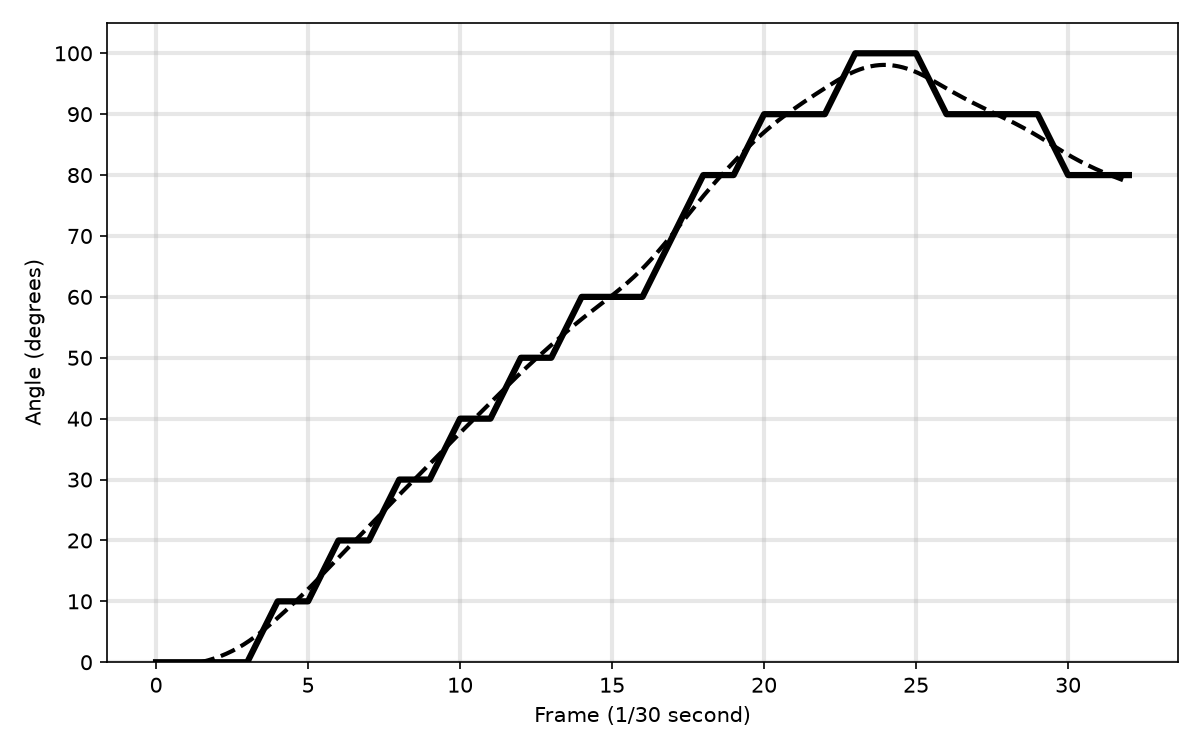
\includegraphics[width=1\textwidth]{graphics/results/actuation_line.png}
    \caption{Braccio arm step response}
    \label{fig_re:braccio_step}
\end{figure}

\section{Inverse Kinematics Solver}
The remaining error over time, after running the inverse kinematics solver, is shown in \autoref{fig_re:sqr_err}, while the latency and error per number of iterations is shown in \autoref{fig_re:lat_per_iter} and \autoref{fig_re:err_per_iter} respectively.

\newpage

\begin{figure}[h!]
    \centering
    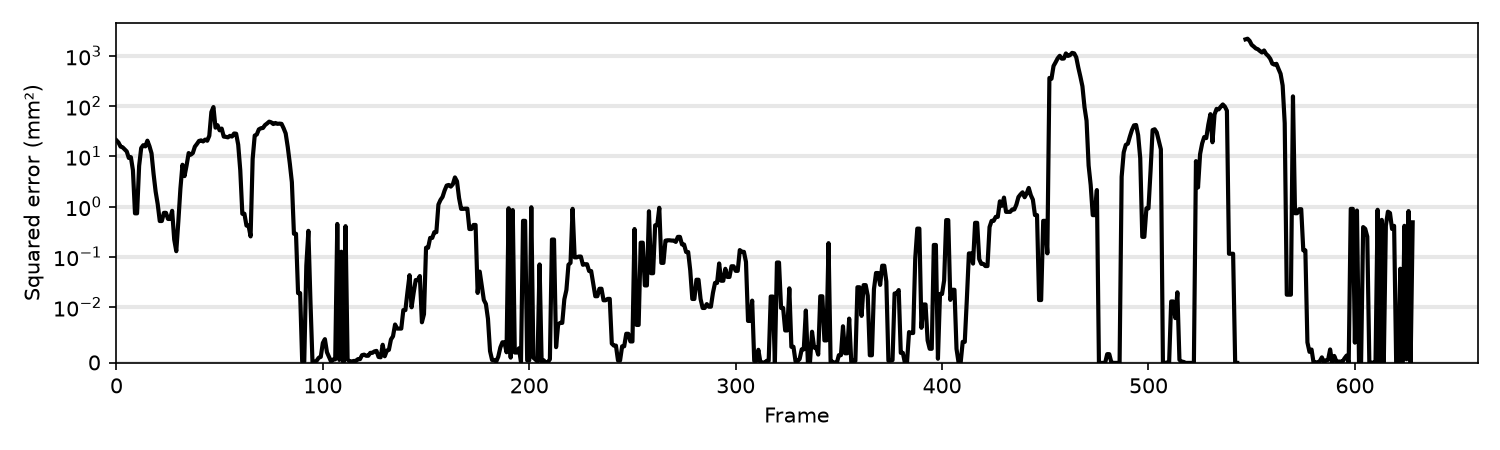
\includegraphics[width=\textwidth]{graphics/results/sqr_err.png}
    \caption{Squared error throughout the teleoperation task}
    \label{fig_re:sqr_err}
\end{figure}

\begin{figure}[h!]
    \centering
    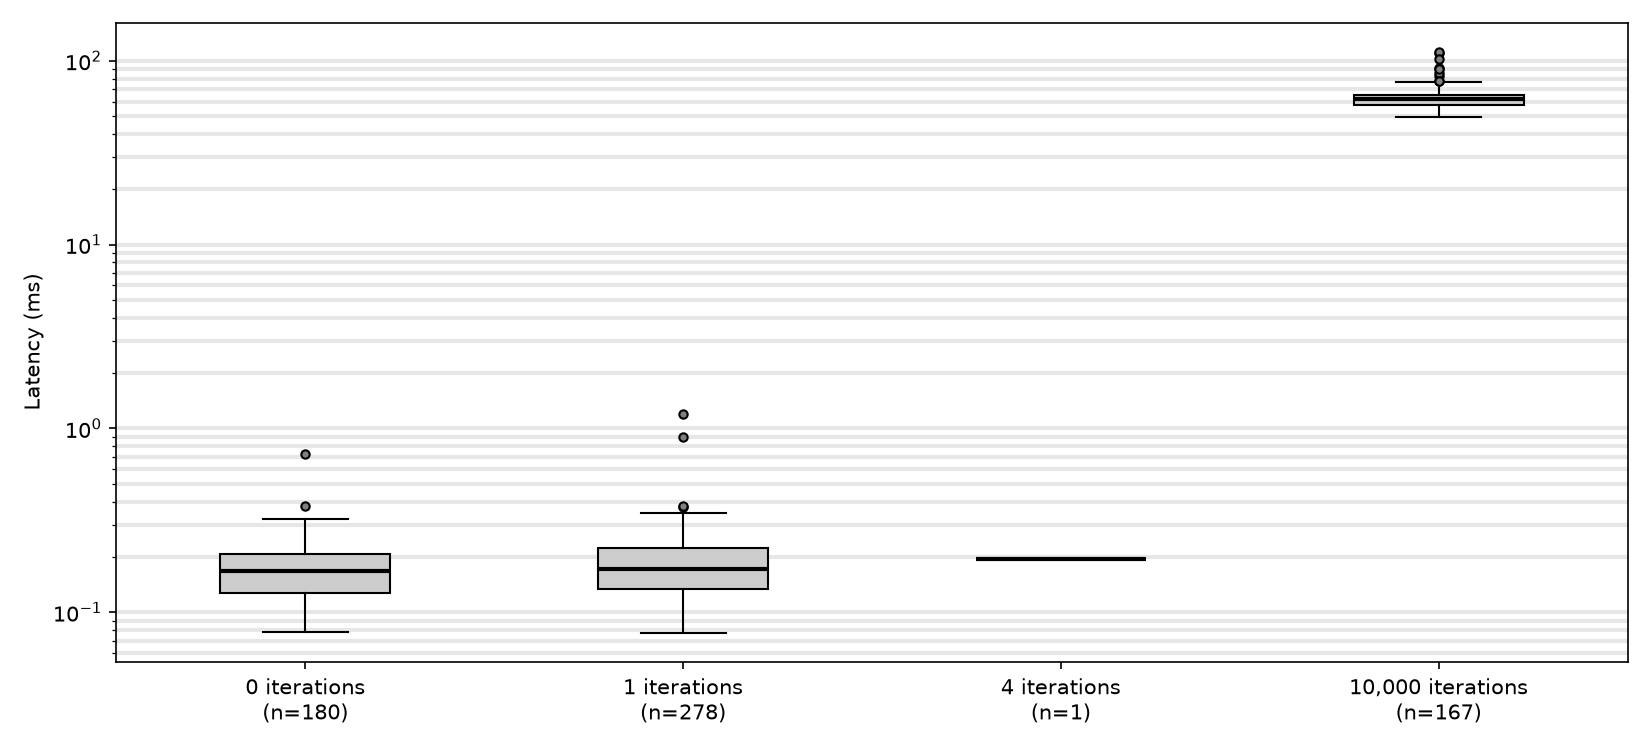
\includegraphics[width=\textwidth]{graphics/results/latency_per_iter.png}
    \caption{Latency per number of iterations}
    \label{fig_re:lat_per_iter}
\end{figure}

\begin{figure}[h!]
    \centering
    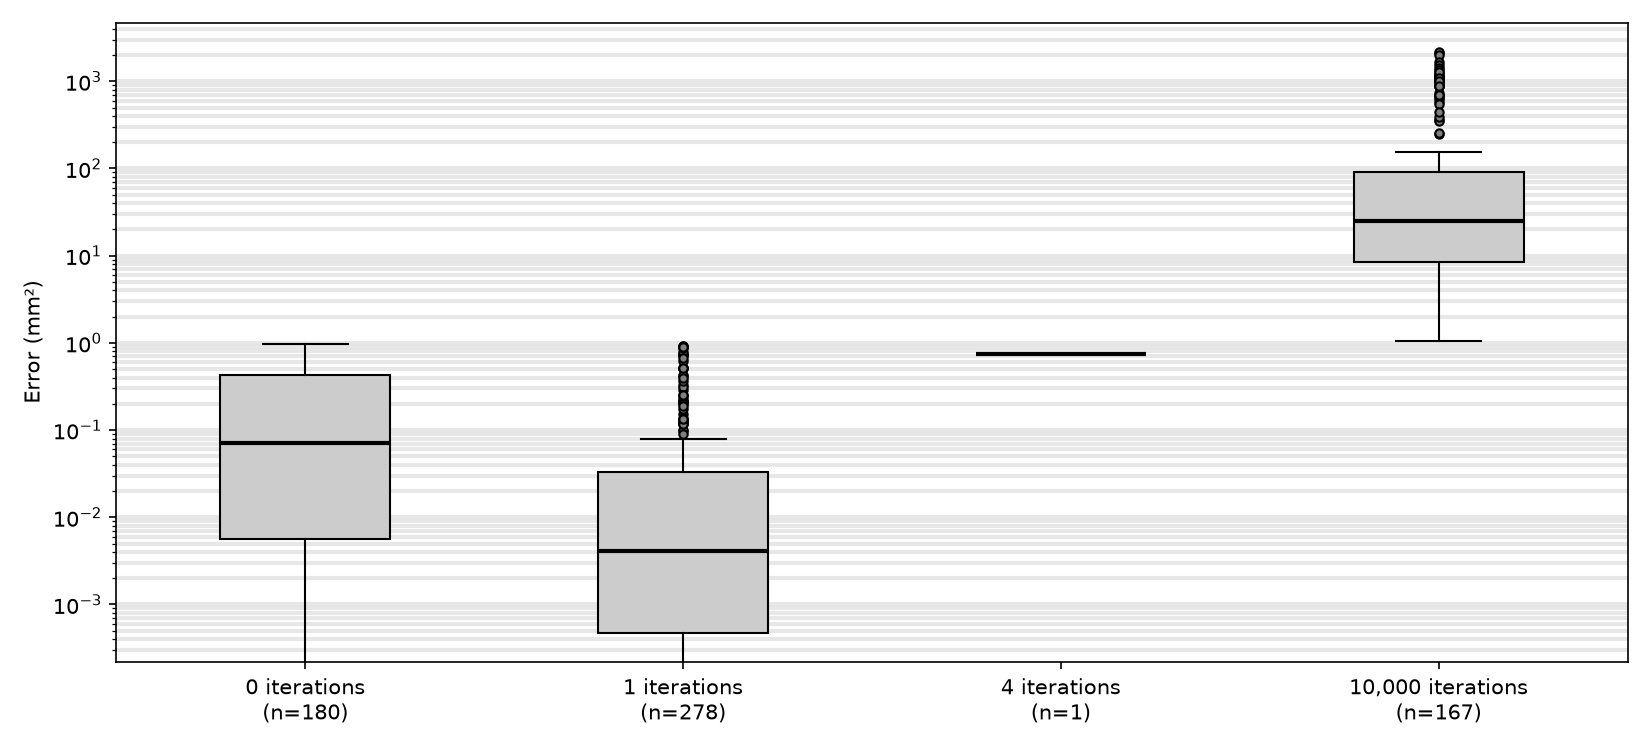
\includegraphics[width=\textwidth]{graphics/results/error_per_iter.png}
    \caption{Squared error per number of iterations}
    \label{fig_re:err_per_iter}
\end{figure}

\chapter{Discussion}\label{ch:dis}

% Here is what the results mean and how they tie to existing literature...

% Discuss the relevance of your results and how they fit into the theoretical work you described in your
% literature review.

\section{Latency}
As seen in \autoref{fig_re:latency_boxplot} and \autoref{tab_re:latency_table}, the primary contributor of latency in the overall system is the exponential smoothing, contributing 88.3\% of the total latency. This brings the total latency to $1.17\pm 0.0425$ seconds.

This is significantly slower than other teleoperation systems. Mongardi \textit{et al.} \cite{bib:braccio_armband_demo} achieve a total latency of 300ms, while Chen \textit{et al.} \cite{bib:teleoperation_TeleopLab} make their robotic manipulator have a motion-latency of only 10ms. However, being faster has a risk of more aggressive movements, which can be hazardous when dealing with industrial robotic manipulators, like in the case of TeleopLab \cite{bib:teleoperation_TeleopLab}. The trade-off between speed and safety remains to be investigated.

The latency due to the networking subsystem (DTLS and UART communication) is $45.677$ms, which is comparable to MediaPipe's landmarking latency of $61$ms. Excluding the exponential smoothing, the networking subsystem contributes $33.51\%$ to the remaining latency. This would be a significant portion.\\
The Braccio was controlled over a relatively fast home network, making the packet travel-time smaller than what it would be in a practical application. The latency due to packets having to travel through the internet will vary significantly, depending on the distance between the operator and slave, reaching latencies upward of $150$ms \cite{bib:world_wide_ping}. This is a factor that could not be expressed in the experiments of the project, and may dwarf the latency of the encryption and decryption (encompassed by the transmission and reception).

The step response of the Braccio has an overshoot of about 10\degree. Exponential smoothing can't inherently introduce overshoot, so this behaviour likely comes from the inertia of the Braccio's arm.\\
The settling point is also below the setpoint. Each linkage in the Braccio isn't held tightly in position and has a bit of wiggle room. This means the arm is able to "sag" due to the effects of gravity, which appears to happen in the video footage.


\newpage
\section{Inverse Kinematics Solver}
The IK solver did not return a variety of iterations. Instead, the algorithm either:
\begin{itemize}[nosep]
    \item Used no iterations (occurred 180 times)
    \item Used 1 iteration (occurred 278 times)
    \item Used 4 iterations (an outlier, occurring once)
    \item Used the maximum 10,000 iterations (occurred 167 times)
\end{itemize}
From the performance of the overall system and the fact that the IK solver passes all ATPs, it's clear that the algorithm \textbf{does} return reasonable solutions. This implies that the algorithm rarely needs more than one iteration to find a solution, otherwise struggles to converge (either due to FABRIK's difficulty with precision or impossible target).

This is supported by the behaviour of the total error throughout the teleoperation task, seen in \autoref{fig_re:sqr_err}. There is no clear convergence behaviour (such as a decaying exponential) that would suggest that the algorithm needs more than 10,000 iterations to converge. Instead, the error fluctuates, possibly due to the nature of the target being fed into the algorithm.\\
Because the target encompasses both position and direction, impossible targets are easy to find, hence yielding errors that can't be reduced. This can be seen when the operator places their hand near the edge of the Braccio's range of motion, and faces it downwards. For the Braccio to meet the positional requirement, it must extend its arm to the maximum length, but this causes the directional requirement to be failed.

For shorter amounts of iterations, the IK solver creates significantly less latency; around $0.2$ms, which can be seen in \autoref{fig_re:lat_per_iter}. This is on par with other IK solvers, where solution times ranges from $0.03$ms to $3.45$ms \cite{bib:TRAC_IK}. This comparison isn't completely fair, because other IK solvers typically aim for more precision ($10^{-6}$mm). After one iteration, the current implementation typically reduces the error below $0.1\text{mm}^2$, as shown in \autoref{fig_re:err_per_iter}.\\
The current implementation would benefit from checking if convergence is failing and then deciding to terminate early.

\section{Cybersecurity}
The current implementation shows some successful defences against cyber attacks. In practice, this implementation is far from a secure system. Current vulnerabilities include, but are not limited to:
\begin{enumerate}[nosep]
    \item Side channel attacks
    \item DoS attacks (untested)
    \item Jamming
    \item Physical attacks, such as glitch attacks
    \item Reprogramming or reading the firmware
    \item Any vulnerabilities on the operator-side device
    \item Social engineering
\end{enumerate}

\chapter{Conclusions}\label{ch:conc}

% These are the conclusions from the investivation and how the investigation changes things in this field or contributes to current knowledge...

% Draw suitable and intelligent conclusions from your results and subsequent discussion.

A full teleoperation pipeline with non-intrusive user readings and  security conscious networking was successfully implemented, although with many limitations.

The final implementation failed to make use of the third dimension of space, thereby limiting the range of tasks the teleoperated slave can accomplish.

The total latency of the slave's response was slower than implementations in existing literature, primarily due to the low-pass filtering done to the Braccio's movements. The inverse kinematics solver has the potential to match the speed of other implementations, but suffers from impossible targets.

The cybersecurity conscious networking subsystem did not significantly impede on the overall system's performance, demonstrating a way to partially secure network traffic in resource constrained systems, such as an ESP32. Many other vulnerabilities still exist.

\chapter{Recommendations}

% Make sensible recommendations for further work.

This paper only evaluates the kinematic mapping software with functional metrics, but does not provide direct insight into its intuitiveness. I would like to see the kinematic mapping software evaluated on intuitiveness, likely using the \textit{completion rate} and \textit{completion time} of teleoperation tasks, performed by novice operators. These metrics are used to evaluate intuitiveness in other teleoperation systems \cite{bib:teleoperation_intuitive_using_MediaPipeHands}\cite{bib:teleoperation_continuous_space}\cite{bib:teleoperation_continuous_space_2}.

Bilateral teleoperation is where the operator receives tactile feedback from the slave limb. This can improve intuitiveness, but is not explored in this paper. Future work may introduce tactile feedback into the system, similar to some other teleoperation systems \cite{bib:teleoperation_surgery}\cite{bib:teleoperation_survey}.

Path tracking is a natural next step when discusses inverse kinematics. The kinematic mapping software can be extended to solve for trajectories, in cases where autonomous movement is required or when setpoints are infrequent.
\bibliographystyle{IEEEtran}
\bibliography{
    bibliography/teleoperation.bib,
    bibliography/kinematic_mapping.bib,
    bibliography/inverse_kinematics.bib,
    bibliography/computer_vision.bib,
    bibliography/network.bib,
    bibliography/tools.bib
}
\appendix
\chapter{Additional Files and Schematics}

Add any information here that you would like to have in your project but is not necessary in the main
text. Remember to refer to it in the main text. Separate your appendices based on what they are for
example. Equation derivations in Appendix A and code in Appendix B etc.

\textbf{IMPORTANT:} Appendix A (see the table below) should provide a summary of how you have met the GAs associated with the course, and where in the report the evidence can be found.

If you have used AI in writing your report, you need to provide details in one of the appendices of how you used it.

If appropriate, in a subsequent appendix, provide a link to any GitHub repository where the code and additional materials for your project can be found.

\begin{center}
\begin{tabular}{||p{2em} |p{15em} |p{20em}||}
 \hline
 \textbf{GA} & \textbf{Requirement} & \textbf{Justification and section in the report}  \\ [0.5ex] 
 \hline\hline
 1 & Problem-solving & Description here  \\ 
 \hline
 4 & Investigations, experiments and data analysis & Description here  \\
 \hline
 5 & Use of engineering tools & Description here \\
 \hline
 6 & Professional and technical communication (Long report) & Description here \\
 \hline
 8 & Individual work & Description here \\
 \hline
 9 & Independent learning ability & Description here \\ [1ex] 
 \hline
\end{tabular}
\end{center}

\chapter{Addenda}

\section{Ethics Forms}
}
\end{document}
